\documentclass{report}
\usepackage[utf8]{inputenc}
\usepackage{graphicx}
\usepackage{longtable}
\usepackage{array}
\usepackage{caption}
\usepackage{mathtools}
\usepackage{listings}

\begin{document}
\section{Analysis}
\subsection{Comparison to the previous experiment}
To calculate the validity of the results, two methods will be used. An analysis of the trend line will be done, and the Pearson correlation will be used. To calculate the trend line, the following equations are used:\\

~\\Slope = 
\begin{flalign*}
\hspace*{-5cm}\alpha = \frac{n\sum(xy)-\sum(x)\sum(y)}{n\sum(x^2)-(\sum(x))^2}
\end{flalign*}
~\\ Intercept =
\begin{flalign*}
\hspace*{-5cm}\beta = \frac{\sum(y)-\alpha\sum(x)}{n}
\end{flalign*}
~\\ Trend line =
\begin{flalign*}
\hspace*{-5cm}y = \alpha x + \beta
\end{flalign*}

~\\ Figure ~\ref{fig:Ex1Combined}, ~\ref{fig:Ex2Combined} and ~\ref{fig:Ex3Combined} show graphs of both data sets combined. Table ~\ref{table:SlopeInt} shows every experiments slope and intercept, and also the ticktime where the first TF loss would be $>$ 1, and how much the ticktime would have to increase after that to be $+$ 1 TF again.

\begin{figure}[!htbp]
	\centering
	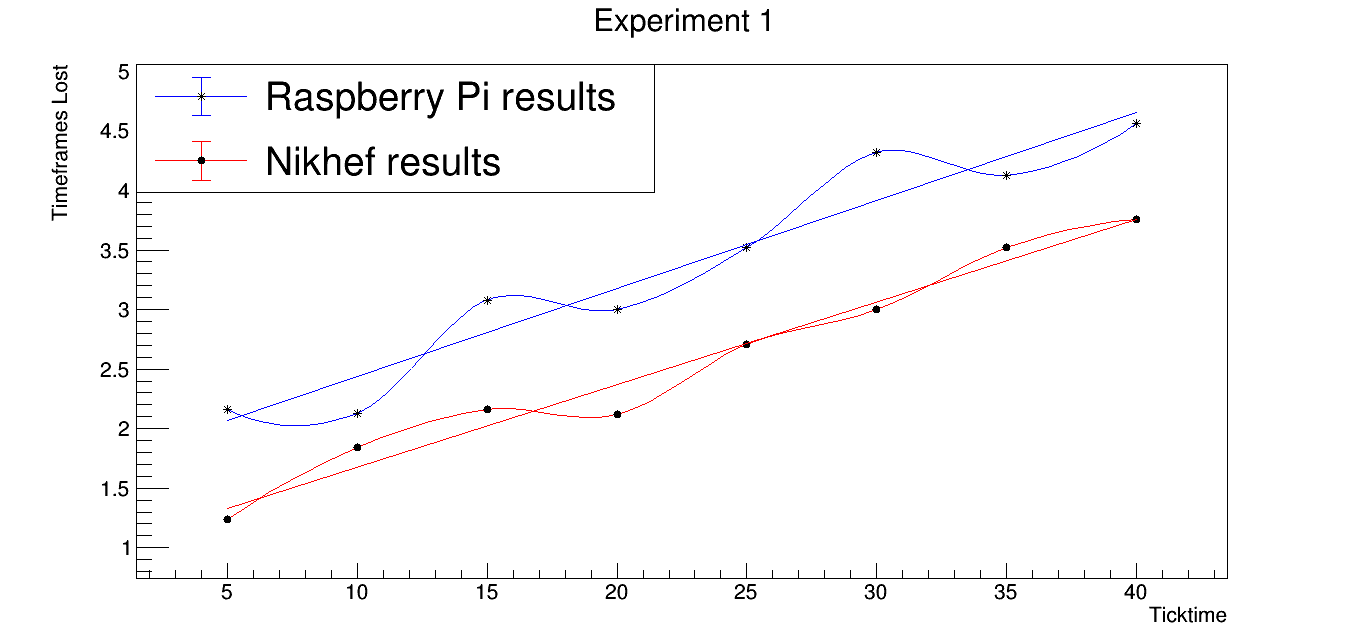
\includegraphics[width=\textwidth,height=\textheight,keepaspectratio]{./graphics/ex1_combined.png}
	\caption{Combined results Experiment 1}
	\label{fig:Ex1Combined}
\end{figure}
\begin{figure}[!htbp]
	\centering
	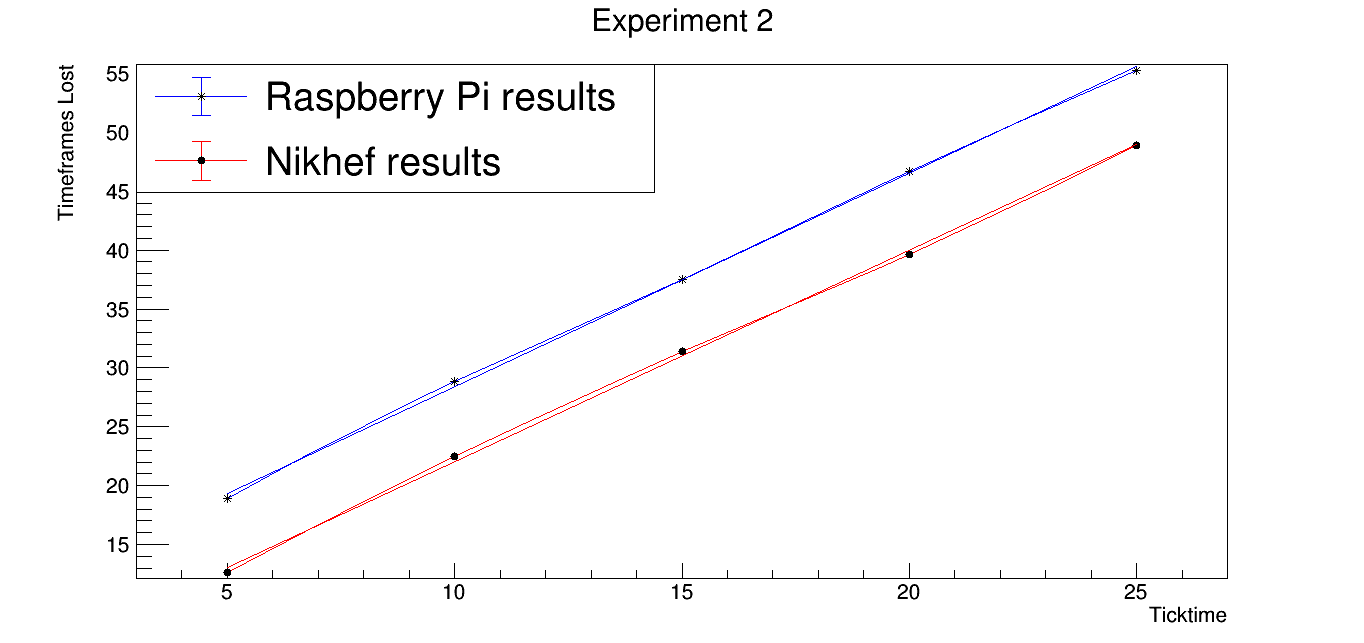
\includegraphics[width=\textwidth,height=\textheight,keepaspectratio]{./graphics/ex2_combined.png}
	\caption{Combined results Experiment 2}
	\label{fig:Ex2Combined}
\end{figure}
\begin{figure}[!htbp]
	\centering
	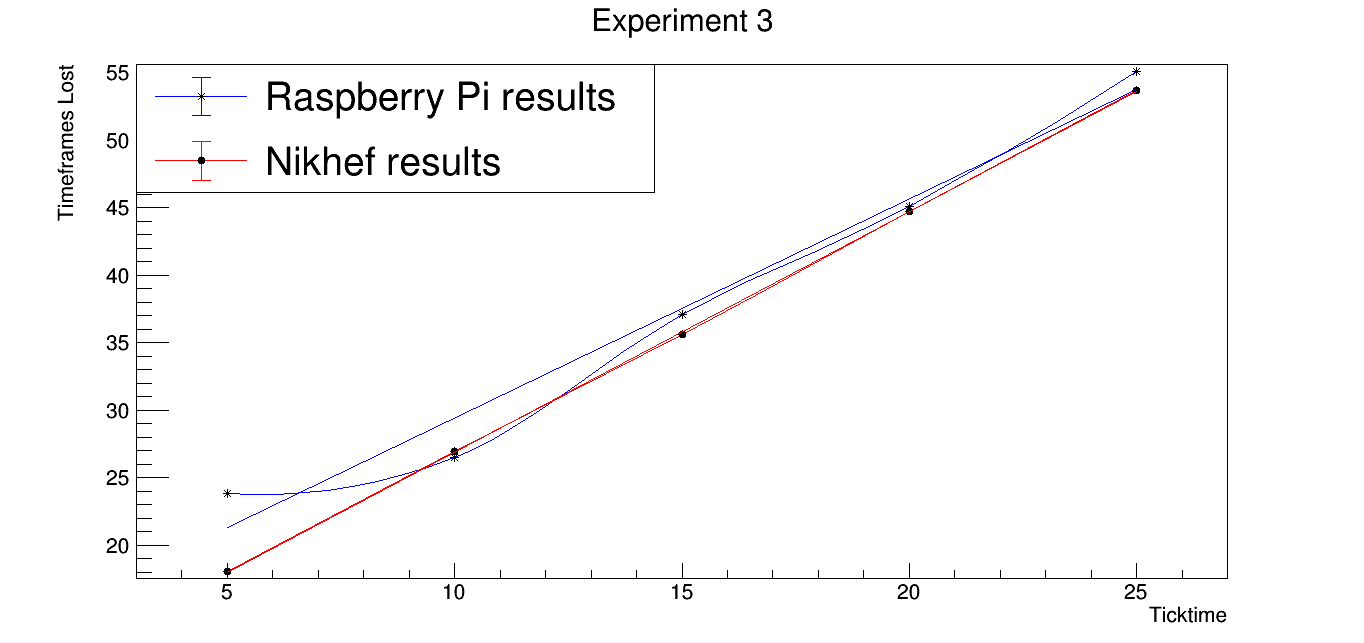
\includegraphics[width=\textwidth,height=\textheight,keepaspectratio]{./graphics/ex3_combined.png}
	\caption{Combined results Experiment 3}
	\label{fig:Ex3Combined}
\end{figure}

\begin{table}[!htbp]
\resizebox{\textwidth}{!}{\begin{tabular}{| >{\centering}m{2cm} | >{\centering}m{2cm} | >{\centering}m{2cm} | >{\centering}m{2cm} | >{\centering}m{2cm} | >{\centering}m{2cm} | >{\centering}m{2cm} |}
\hline
& Slope Pi & Intercept Pi & Slope Nikhef & Intercept Nikhef & First $>$ 1 & Next $+$ 1 \tabularnewline \hline
Experiment 1 & 0.074 & 1.7 & 0.069 & 0.982 & 64 & 222 \tabularnewline \hline
Experiment 2 & 1.810 & 10.305 & 1.794 & 4.077 & - & 64 \tabularnewline \hline
Experiment 3 & 1.622 & 13.216 & 1.783 & 9.072 & - & 6 \tabularnewline 
\hline
\end{tabular}}
\caption{Slope and Intercepts combined experiments}
\label{table:SlopeInt}
\end{table}

\newpage

~\\These figures show that the for the first experiment, the ticktime has to increase by 222 in order for the difference in TF loss be $+$ 1 again. For experiment two this is 64, and for experiment 3 it's the other way around, where the results from Nikhef will end up higher than from the Raspberry Pi. The first time this happens is at Ticktime 32. The point where it swaps is at ticktime 26. 
\end{document}